Gell--Mann--Low formula has been made to work \cite{pct-app-61,pct-app-62,pct-app-60}.  These
results show that theories exist satisfying the axioms and having infinite
renormalizations, and furthermore, that non-trivial theories can exist in
space-times of at least three dimensions.

Unfortunately, none of the papers gives a complete answer to the question of
the existence of solutions for typical four-dimensional theories, say,
$(\varphi^4)_4$ or the quantum electrodynamics of spin $\tfrac12$ particles.
The phenomenon of charge renormalization, which is unavoidable for the
treatment of such renormalizable but not superrenormalizable theories, has as
yet not been treated in constructive field theory.  It is clearly one of the
main roadblocks in the way of a completely satisfactory answer to the
question of the existence of non-trivial theories.  There are many
intriguing but so far inconclusive investigations in this area, of which we
mention only \cite{pct-app-63,pct-app-64}.

Thus, in our opinion, \emph{constructive quantum field theory has provided a
very satisfactory solution of the Main Problem; but, so far, only for
super-renormalizable theories in space-times of dimension $\leq 3$.}

\subsection*{Local Algebras and Superselection Sectors}
\phantomsection
\addcontentsline{toc}{subsection}{Local Algebras and Superselection Sectors}
\label{sec:appendix-local-algebras}

In the early 1960s, an alternative version of the foundations of
relativistic quantum field theory was developed \cite{pct-app-65}, based on the use of
algebras of bounded operators.  Although in principle this formalism should
be roughly equivalent to the axiomatic field theory described in this book,
it turned out to be very difficult to obtain a smooth connection between the
two, and so it has been developed in parallel with the quantum theory of
fields \cite{pct-app-66}.  For certain general theoretical purposes, the local algebra
formalism turned out to be very natural.  In particular, it yields a theory
of superselection rules which throws new light on the axioms discussed in
this book.  In the following we sketch this special line of argument and
refer the reader to \cite{pct-app-67} for a systematic account of the algebraic approach
and a bibliography.

The basic objects of the local algebra formalism are $C^*$ algebras,
$\mathcal A(\mathcal O)$, associated with bounded open sets, $\mathcal O$, in
space-time.  These algebras are supposed to form a net in the sense that
\begin{equation*}
  \mathrm{I.}\qquad
  \mathcal O_1\subseteq\mathcal O_2
  \quad\Longrightarrow\quad
  \mathcal A(\mathcal O_1)\subseteq\mathcal A(\mathcal O_2).
\end{equation*}

The relativistic invariance of the theory is expressed as
\begin{equation*}
  \begin{aligned}
    \mathrm{II.}\qquad
    &\text{There exists a representation, $\alpha$, of the Poincar\'e group}\\
    &\text{by automorphisms of $\mathcal A$:}\qquad
      \{a,\Lambda\}\longmapsto\alpha(a,\Lambda)
  \end{aligned}
\end{equation*}

\begin{equation*}
  \begin{aligned}
    &\text{such that if $A\in\mathcal A(\mathcal O)$, then}\\
    &\qquad\alpha(a,\Lambda)(A)\in\mathcal A(\Lambda\mathcal O+a).
  \end{aligned}
\end{equation*}

It therefore makes sense to speak of $\bigcup_{\mathcal O}\mathcal A(\mathcal
O)$ and its norm closure, $\mathcal A$, which is called the
\emph{quasilocal algebra}.  The $\mathcal A(\mathcal O)$ algebra is also
supposed to satisfy the analogue of local commutativity
\begin{equation*}
  \mathrm{III.}\qquad
  \mathcal O_1\ \text{space-like separated from}\ \mathcal O_2
  \quad\Longrightarrow\quad
  \mathcal A(\mathcal O_1)\subseteq\mathcal A(\mathcal O_2)',
\end{equation*}
where the prime indicates the commutant in $\mathcal A$.

One can now define, in terms of these algebraic objects, the second
fundamental notion of this theory, the notion of \emph{state}.  A state, $\rho$,
is a complex-valued linear function on the quasilocal algebra $\mathcal A$:
\begin{equation*}
  \rho(\lambda A)=\lambda\rho(A)
  \qquad\text{for all $\lambda\in\mathbb C$ and $A\in\mathcal A$,}
\end{equation*}

\begin{equation*}
  \rho(A+B)=\rho(A)+\rho(B),
\end{equation*}
which is positive in the sense that
\begin{equation*}
  \rho(A^*A)\geq0
\end{equation*}
and normalized in the sense that
\begin{equation*}
  \rho(\mathbf 1)=1,
\end{equation*}
where $\mathbf 1$ is the identity in $\mathcal A$.  (We are tacitly
assuming all our $C^*$ algebras contain an identity.)  A state is said to be
\emph{invariant} under the Poincar\'e group if
\begin{equation*}
  \rho(A)=\rho\bigl(\alpha(a,\Lambda)(A)\bigr)
\end{equation*}
for all Poincar\'e transformations $(a,\Lambda)$ and all $A\in\mathcal A$.
The importance of the notion of state is that a state determines a
representation of $\mathcal A$ via the so-called GNS construction \cite{pct-app-68}.

\begin{theorem*}
If $\mathcal A$ is a $C^*$ algebra with unit and $\rho$ a state of $\mathcal A$,
then there exists a Hilbert space $\mathcal H_\rho$, a vector
$\ket{\Psi_\rho}\in\mathcal H_\rho$, and a representation, $\pi_\rho$, of
$\mathcal A$ by bounded operators in $\mathcal H_\rho$ such that
\begin{equation}
  \rho(A)=\matrixel{\Psi_\rho}{\pi_\rho(A)}{\Psi_\rho}
  \qquad\text{for all $A\in\mathcal A$,}
  \tag{1}\label{eq:app-gns-1}
\end{equation}

\begin{equation}
  \ket{\Psi_\rho}\text{ is a cyclic vector for }\pi_\rho(\mathcal A).
  \tag{2}\label{eq:app-gns-2}
\end{equation}

Furthermore, if $\rho$ is invariant under a group $G$ in the sense that there
is a representation $g\mapsto\alpha_g$ of $G$ by automorphisms
of $\mathcal A$
such that $\rho(A)=\rho(\alpha_g(A))$, then there exists a representation
$U_\rho(g)$ of $G$ by unitary operators in $\mathcal H_\rho$ such that
\begin{equation}
  U_\rho(g)\ket{\Psi_\rho}=\ket{\Psi_\rho},
  \tag{3}\label{eq:app-gns-3}
\end{equation}

\begin{equation}
  \pi_\rho(\alpha_g(A))
  =U_\rho(g)\pi_\rho(A)U_\rho(g)^{-1}.
  \tag{4}\label{eq:app-gns-4}
\end{equation}
\end{theorem*}

Thus, the GNS construction shows that to pass from the purely algebraic
notions associated with the quasilocal algebra to a concrete representation,
one need only choose a state.  If the state is invariant, it will determine a
representation in which there is an invariant vector representing the
vacuum.  If the state is not invariant, it may still be \emph{covariant},
i.e., there may exist in $\mathcal H_\rho$ a unitary representation of the
Poincar\'e group $\{a,\Lambda\}\mapsto U(a,\Lambda)$ such that (4) holds for
all $g$ in the Poincar\'e group.  It turns out that not all covariant states
can be regarded as physically realizable.  For example, the unitary
representation of the Poincar\'e group $U_\rho(a,\Lambda)$ may not satisfy
the spectral condition.  However, even after the covariant states have been
winnowed to leave only those that may reasonably be regarded as physically
realizable, it may happen that there are inequivalent representations,
representations that differ in their physical predictions.  For example,
they may yield a different mass and spin spectrum.  What is the significance
of such physically inequivalent representations?  The answer proposed in
\cite{pct-app-65} is that the theory in question has \emph{superselection rules}, and the
classes of physically admissible inequivalent representations label the
coherent subspaces (see Chapter \ref{ch:relativistic-transformation-laws}, pp.~5--6, for a discussion of
superselection rules).

The general theory of \cite{pct-app-65} was further developed in a more specific context
in \cite{pct-app-69,pct-app-70,pct-app-71} but the theory as it stood did not determine how the phenomena
associated with unitary inequivalent representations of the algebras of
observables would appear in concrete Lagrangian field theories.

The first example analyzed in detail was the theory of a massless scalar
field in two-dimensional space-time \cite{pct-app-72}.  The main motivation for this work
was to show, using the ideas of the theory of local algebras, that a precise
mathematical meaning can be given to proposals of Skyrme on the construction
of fermion fields from boson fields \cite{pct-app-73}.

Skyrme's idea was that in the theory of a neutral scalar boson field
satisfying the sine-Gordon equation
\begin{equation*}
  \Box\varphi+\frac{\alpha_0}{\beta}:\!\sin\beta\varphi(x)\!:=0.
\end{equation*}
there are particle-like excitations which should be fermions.  Viewed in the
light of what has come after, his exploratory calculations seem
extraordinarily prescient.

What was done in \cite{pct-app-72} was to consider the very special case in which
$\alpha_0=0$.  The first step was to construct a Fock space representation of
the scalar field $\varphi$ satisfying
\begin{equation*}
  \Box\varphi(x)=0.
\end{equation*}

To avoid troubles with infrared divergences the test functions for the field
were restricted to those elements of $\mathcal S$ whose Fourier transforms
vanish at the origin.  Associated with this field $\varphi$ are two
conserved currents
\begin{equation*}
  \sqrt{\pi}\,j^\mu(x)=-\epsilon^{\mu\nu}\partial_\nu\varphi(x)
  \qquad\text{and}\qquad
  j^{5\mu}(x)=\epsilon^{\mu\nu}j_\nu(x)
\end{equation*}
whose corresponding charges
\begin{equation*}
  Q=\int\dd x\,j^0(x)
  \qquad\text{and}\qquad
  Q^5=\int\dd x\,j^{50}(x)
\end{equation*}

\begingroup
\emergencystretch=1em
\raggedright
vanish in the Fock representation.  However, the local algebras constructed
from $\varphi$ have a two-parameter family of representations for which these
charges take all real values.  If one selects the subset of the
representations with integer charge\linebreak
$\{\Pi_{n_1,n_2}\text{ in the Hilbert space}$%
$\,\mathcal H_{n_1,n_2};$%
$\ n_1,n_2\text{ integers}\}$
and forms the direct sum
\par
\endgroup
\begin{equation*}
  \bigoplus_{n_1,n_2\in\mathbb Z}\Pi_{n_1,n_2}
  \quad\text{in the direct-sum Hilbert space}\quad
  \mathcal H=\bigoplus_{(n_1,n_2)\in\mathbb Z^2}\mathcal H_{n_1,n_2},
\end{equation*}
then one can define charged fermion operators in $\mathcal H$, which
decrease one or the other of the charges by one unit.  At first, it was not
recognized that these fermion operators may be chosen to be the two
components of a fermion field satisfying the equations of the massless
Thirring model, even though the natural occurrence of a free massless boson
field\begingroup
\renewcommand{\thefootnote}{\ensuremath{\dagger}}%
\footnote{%
The currents of the Thirring model are obtained from the free currents,
above, by an automorphism mixing $j$ and $j^5$.
}\endgroup
in the Thirring model had been known for some time \cite{pct-app-74}.  However, by 1973,
the construction had been explicitly carried out and recognized as a
rigorous version of Skyrme's idea for the case in which $\alpha_0=0$ \cite{pct-app-74,pct-app-75}.

For $\alpha_0\ne0$, it was \cite{pct-app-77} that conveyed the decisive insight.  It was
pointed out there that the sine-Gordon theory with general $\alpha_0$ is a
subtheory of a theory of fermions described by a charged two-component
spinor field which satisfies the equations of the so-called massive Thirring
model
\begin{equation*}
  (-\ii\gamma^\mu\partial_\mu+m)\psi
  =g\,:\!\bar\psi\gamma^\mu\psi\!:\,\gamma_\mu\psi.
\end{equation*}
$\psi$ is related to $\varphi$ by
\begin{equation*}
  :\!\bar\psi(x)\gamma^\mu\psi(x)\!:
  =-\frac{\beta}{2\pi}\epsilon^{\mu\nu}\partial_\nu\varphi,
  \qquad
  :\!\bar\psi(x)\psi(x)\!:
  =-\frac{\alpha_0}{\beta^2m}:\!\cos\beta\varphi\!:\,.
\end{equation*}
where $4\pi/\beta^2=1+g/\pi$.

In the massive Thirring model the charge $Q$ defined (with a slightly
different normalization) as
\begin{equation*}
  Q=\int\dd x\,:\!\bar\psi(x)\gamma^0\psi(x)\!:
\end{equation*}
remains a conserved quantity, but the $Q^5$ of the massless theory has no
conserved analogue.  The Hilbert space of the massive Thirring model is a
direct sum
\begin{equation*}
  \mathcal H=\bigoplus_q\mathcal H_q
\end{equation*}
of subspaces $\mathcal H_q$ where $q$ are the eigenvalues of $Q$, integer
multiples of the charge of a single fermion.  The Hilbert space of the
sine-Gordon theory is the vacuum sector $\mathcal H_0$ of $\mathcal H$.

The rigorous construction of the new sectors for general $\alpha_0$ and a
range of $\beta$: $0\leq\beta^2\leq2\sqrt{\pi}$ is found in \cite{pct-app-78,pct-app-79,pct-app-80,pct-app-81,pct-app-82}.  The
basic idea is similar to that of \cite{pct-app-72}: one constructs an automorphism of the
local algebra of observables $\mathcal A$ which, roughly described, has the
property
\begin{equation*}
  \lim_{x\to-\infty}
  \matrixel{\Psi}{\alpha_g(\varphi(x))}{\Psi}
  =\lim_{x\to-\infty}\matrixel{\Psi}{\varphi(x)}{\Psi},
\end{equation*}

\begin{equation*}
  \lim_{x\to+\infty}
  \matrixel{\Psi}{\alpha_g(\varphi(x))}{\Psi}
  =\lim_{x\to+\infty}
  \left[\matrixel{\Psi}{\varphi(x)}{\Psi}+g(x)\right]
\end{equation*}
for normalized states $\ket{\Psi}$ of the sine-Gordon theory itself.  Then a
new state $\omega_g$ on the algebra of observables $\mathcal A$ is defined by
\begin{equation*}
  \omega_g(A)=\matrixel{\Omega}{\alpha_g(A)}{\Omega},
\end{equation*}
where $\ket{\Omega}$ is the vacuum of the sine-Gordon theory.  If $g$ is
chosen as an appropriate ``kink'' function approaching $2\pi m/\beta$ as
$x\to+\infty$, where $m$ is an integer, then $\omega_g$ defines a new
$(m\text{-soliton})$ sector.  Unlike the constructions for $\alpha_0=0$,
which are elementary and explicit, those for $\alpha_0\ne0$ are a \emph{tour
de force} of constructive field theory, since one has first to prove the
existence of the solution of the cutoff-free sine-Gordon theory.

The general theory of \cite{pct-app-78,pct-app-79,pct-app-80,pct-app-81} shows that superselection sectors associated
with a ``topological charge'' (such as the
$\beta\int\dd x\,\frac{\partial}{\partial x}\varphi=2\pi m$ just mentioned)
occur in a wide class of theories in two-dimensional space-time, including
pseudo-scalar $Y_2$ and $(\varphi^4)_2$---in fact, whenever the dynamics of
the system results in symmetry breaking with an associated discrete family of
superselection sectors.  These new sectors do not contain new vacuum states;
rather they contain states of new particles stabilized by the topological
charge they carry, together with composite states formed of the new particles
and any of the old occurring in the vacuum sectors.  As these papers
emphasize, there are still
a number of non-trivial mathematical problems to be solved before the
scattering theory in the new sectors can be regarded as firmly established.
What is clear is that the reasonable interpretation of the meaning of axiom
IV (asymptotic completeness) has changed as a result of these developments.
If, for example, one considers the $\lambda(\varphi^4)_2$ model, one would
expect asymptotic completeness to hold in the one-phase region of $\lambda$
with scattering states formed from the single-particle states established by
the now standard results of constructive field theory.  (To be sure that
there are not additional bound states one needs deep results on the spectrum
of the theory \cite{pct-app-83,pct-app-84,pct-app-85}.)  However, for $\lambda$ in the two-phase region, one
expects asymptotic completeness to hold only after one has adjoined to the
Hilbert space the new sectors containing a soliton or anti-soliton.

It appears that the sine-Gordon model is not a good example on which to base
arguments for the necessity of this altered interpretation of asymptotic
completeness, because no inelastic processes take place \cite{pct-app-86}.  If that is
indeed the case, meson collisions do not produce soliton--anti-soliton pairs
and the scattering matrix for mesons is unitary in the vacuum sector alone.
Asymptotic completeness would be expected to hold for the theory of the
boson field in the vacuum sector.  On the other hand, for the
$(\varphi^4)_2$ theory in the two-phase region one expects colliding mesons to
produce kink--anti-kink pairs, so the introduction of new sectors would be
necessary to achieve asymptotic completeness.

The existence of new sectors of the $(\varphi^4)_2$ theory in the two-phase
region raises some problems of interpretation: What should the Hilbert space
of the theory be?  Is the resulting theory a quantum field theory in the
sense of the definitions of this book?

To answer the first question it is necessary to examine the physical
properties of the various sectors.  The two vacuum sectors $\mathcal H_{0+}$
and $\mathcal H_{0-}$ are distinguished by
$\langle\varphi(x)\rangle_{0+}>0$ and $\langle\varphi(x)\rangle_{0-}<0$ with
$\langle\varphi(x)\rangle_{0+}=-\langle\varphi(x)\rangle_{0-}$ constant in
$x$.  There is also a soliton (kink) sector, $\mathcal H_s$,
characterized by
\begin{equation*}
  \lim_{x\to\pm\infty}\langle\varphi(x)\rangle_s
  =\langle\varphi(x)\rangle_{0\pm}
\end{equation*}
and an anti-soliton sector, $\mathcal H_{\bar s}$, characterized by
\begin{equation*}
  \lim_{x\to\pm\infty}\langle\varphi(x)\rangle_{\bar s}
  =\langle\varphi(x)\rangle_{0\mp}.
\end{equation*}

Notice that the soliton and anti-soliton states are not translation invariant.
However, it turns out that they are covariant.  The iteration
of the automorphism associated with the soliton, $s$, on the vacuum sector
$\mathcal H_{0,\pm}$ yields a state which again lies in $\mathcal H_{0,\pm}$
(symbolically $s^2\sim e$, in the group of automorphisms) and similarly for
$\bar s$: $\bar s^2\sim e$.  On the other hand, the composition,
$s\mathbin\circ\bar s$ of the automorphisms $s$ and $\bar s$ applied on
$\mathcal H_{0,\pm}$ yields a state in $\mathcal H_{0,\mp}$.  An intuitive
picture of these facts can be obtained from Figure \ref{fig:A-3}.

The standard approach to the interpretation of the four sectors
$\mathcal H_{0+}$, $\mathcal H_{0-}$, $\mathcal H_s$, and $\mathcal H_{\bar s}$
would regard the two vacuum sectors $\mathcal H_{0+}$ and $\mathcal H_{0-}$ as
physical alternatives and would attempt to adjoin $\mathcal H_s$ or
$\mathcal H_{\bar s}$, or both, to obtain an asymptotically complete theory.
If, as has been argued in \cite{pct-app-87}, the lowest part of the mass spectrum in
$\mathcal H_s$ is an isolated eigenvalue, one can use the Haag--Ruelle theory
of collisions to prove the existence of kink--anti-kink states in
$\mathcal H_{0+}$ (and in $\mathcal H_{0-}$) which are not meson states.
Thus, to obtain an asymptotically complete theory starting from
$\mathcal H_{0+}$ one has at least to adjoin $\mathcal H_s$ or
$\mathcal H_{\bar s}$ or both, thereby obtaining
\begin{equation*}
  \mathcal H_{0+}\oplus\mathcal H_s
  \quad\text{or}\quad
  \mathcal H_{0+}\oplus\mathcal H_{\bar s}
  \quad\text{or}\quad
  \mathcal H_{0+}\oplus\mathcal H_s\oplus\mathcal H_{\bar s}
\end{equation*}
as state space.  Similarly, starting from $\mathcal H_{0-}$, one has the
three possibilities
\begin{equation*}
  \mathcal H_{0-}\oplus\mathcal H_s
  \quad\text{or}\quad
  \mathcal H_{0-}\oplus\mathcal H_{\bar s}
  \quad\text{or}\quad
  \mathcal H_{0-}\oplus\mathcal H_s\oplus\mathcal H_{\bar s}.
\end{equation*}

The third possibility in each case is distinguished by the existence of a
parity operator; the first two are analogous to theories of neutrinos
without anti-neutrinos in having a particle $s$ or $\bar s$ whose
anti-particle is, in fact, absent but would appear if a parity operator, $P$,
existed and acted on the particle: $Ps=\bar s$.

To make further distinctions among the possibilities it is natural to
associate fields with the particles $s$ (and $\bar s$).  The vacuum,
$\ket{\Omega_{0+}}$, is not a cyclic vector for any of the three possible
Hilbert spaces which contain $\mathcal H_{0+}$, so that to obtain a field
theory it is necessary to adjoin fields which map the vacuum sector into the
other sectors.  No local fields are known which do this, but by following the
ideas of the theory of local algebras, one can obtain fields $s(x)$ and
$\bar s(x)$ which have some weakened locality properties \cite{pct-app-79}.  Namely,
$s(x)$ anti-commutes with $\varphi(y)$ if $y$ is sufficiently far to the
right of $x$ and commutes if it is sufficiently far to the left.  However,
one cannot realize both $s(x)$ and $\bar s(x)$ in any of the six Hilbert
spaces above.  Instead one needs
\begin{equation*}
  \mathcal H_{0+}\oplus\mathcal H_{0-}\oplus\mathcal H_s\oplus\mathcal H_{\bar s}.
\end{equation*}

The reason for this is that $s(x)\bar s(y)\ket{\Omega_{0+}}$ lies in the
subspace $\mathcal H_{0-}$, as it must if the action of $s(x)\bar s(y)$
implements the automorphism $s\mathbin\circ\bar s$.  (See Figure \ref{fig:A-3}.)

% PCT-SOURCE: pdf=210 print=198 kind=figure id=A.3
% Native reconstruction of the state profiles and automorphism arrows on
% source page 198.  The curves are schematic profiles, as in the source.
\begingroup
\renewcommand{\thefigure}{A.3}
\renewcommand{\figurename}{Figure}
\begin{figure}[p]
  \centering
\resizebox{\textwidth}{!}{%
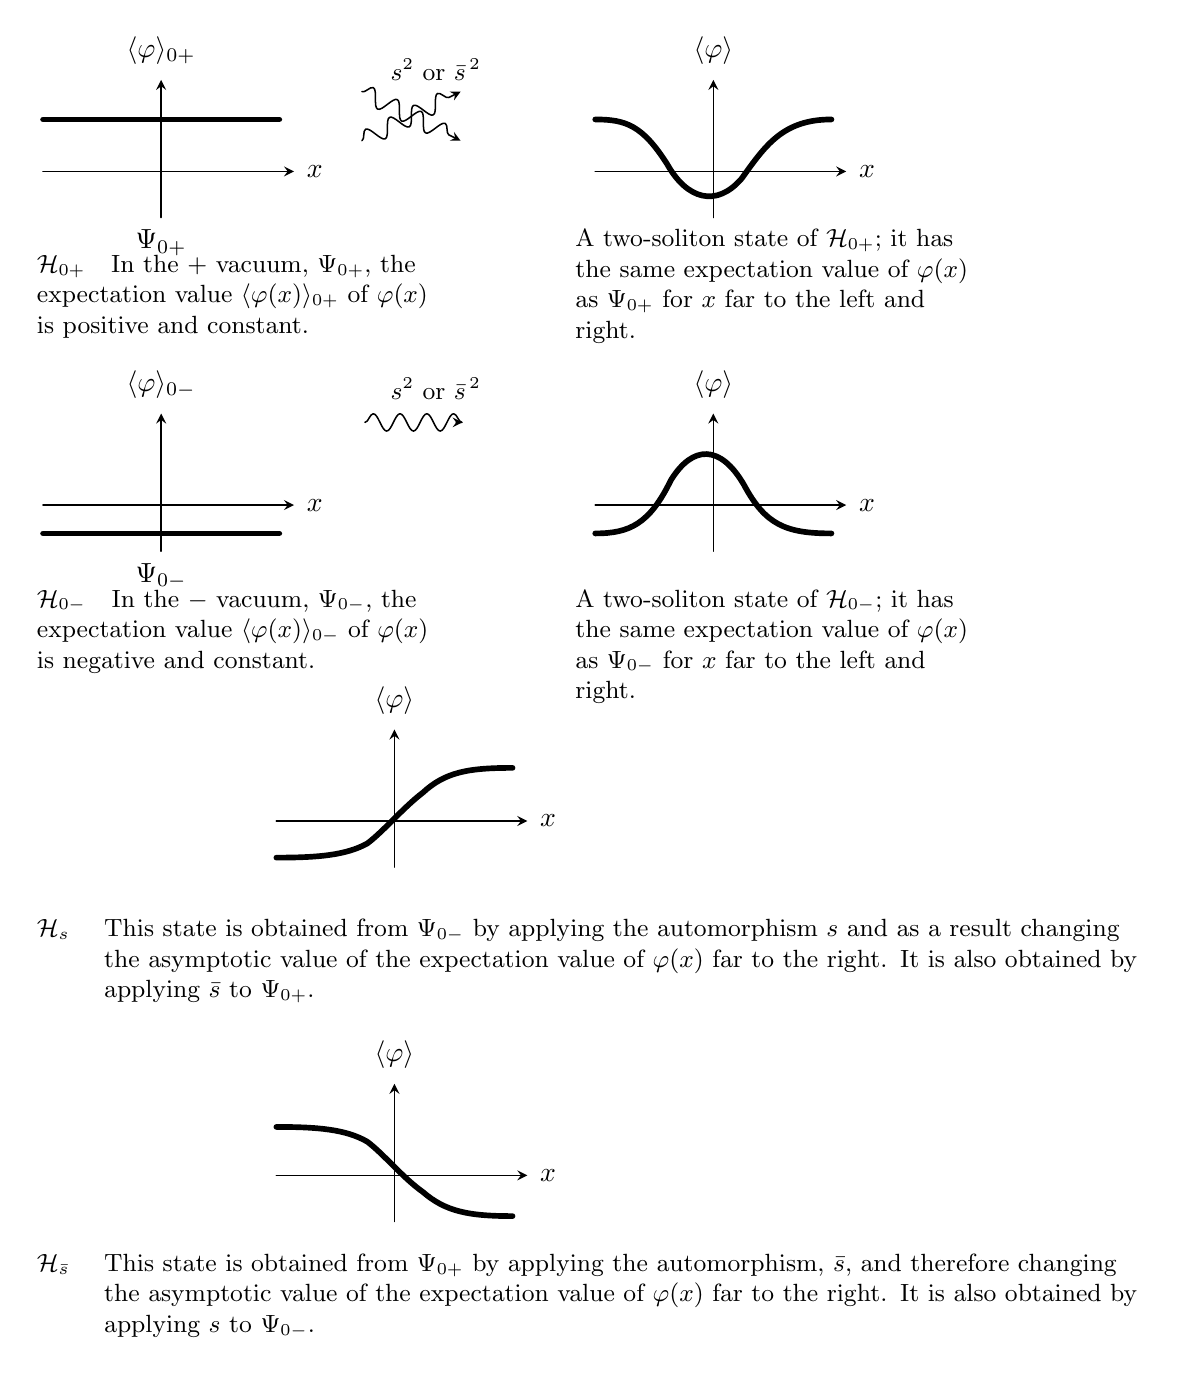
\begin{tikzpicture}[x=.75cm,y=.75cm,>=stealth,line cap=round,
    line join=round]
    % Reusable axes for the four small profiles.
    \newcommand{\pctaxes}[1]{%
      \draw[->,line width=.6pt] (#1-2.0,0) -- (#1+2.25,0)
        node[right=1pt] {$x$};%
      \draw[->,line width=.6pt] (#1, -.78) -- (#1,1.55);%
    }

    % Top-left: the positive vacuum.
    \begin{scope}[shift={(2.35,13.2)}]
      \pctaxes{0}
      \draw[line width=2.05pt] (-2.0,.88) -- (2.0,.88);
      \node[above=2pt] at (0,1.55) {$\langle\varphi\rangle_{0+}$};
      \node[below=1pt] at (0,-.78) {$\Psi_{0+}$};
    \end{scope}
    \node[anchor=north west,text width=5.2cm,align=left,font=\small]
      at (.08,11.95) {$\mathcal H_{0+}$\quad In the $+$ vacuum, $\Psi_{0+}$, the expectation value $\langle\varphi(x)\rangle_{0+}$ of $\varphi(x)$ is positive and constant.};

    % Top-right: a two-soliton profile in the positive sector.
    \begin{scope}[shift={(11.7,13.2)}]
      \pctaxes{0}
      \draw[line width=2.05pt]
        (-2.0,.88) .. controls (-1.48,.88) and (-1.20,.78) .. (-.78,.12)
        .. controls (-.45,-.47) and (.05,-.62) .. (.48,-.12)
        .. controls (.88,.44) and (1.18,.88) .. (2.0,.88);
      \node[above=2pt] at (0,1.55) {$\langle\varphi\rangle$};
    \end{scope}
    \node[anchor=north west,text width=5.15cm,align=left,font=\small]
      at (9.2,12.38) {A two-soliton state of $\mathcal H_{0+}$; it has the same expectation value of $\varphi(x)$ as $\Psi_{0+}$ for $x$ far to the left and right.};

    % The crossed wavy arrows between the first row of panels.
    \node[font=\small] at (7.0,14.92) {$s^2$ or $\bar s^{\,2}$};
    \draw[->,line width=.55pt,decorate,
      decoration={snake,amplitude=.11cm,segment length=.34cm}]
      (5.75,14.55) -- (7.42,13.72);
    \draw[->,line width=.55pt,decorate,
      decoration={snake,amplitude=.11cm,segment length=.34cm}]
      (5.75,13.72) -- (7.42,14.55);

    % Middle-left: the negative vacuum.
    \begin{scope}[shift={(2.35,7.55)}]
      \pctaxes{0}
      \draw[line width=2.05pt] (-2.0,-.48) -- (2.0,-.48);
      \node[above=2pt] at (0,1.55) {$\langle\varphi\rangle_{0-}$};
      \node[below=1pt] at (0,-.78) {$\Psi_{0-}$};
    \end{scope}
    \node[anchor=north west,text width=5.2cm,align=left,font=\small]
      at (.08,6.28) {$\mathcal H_{0-}$\quad In the $-$ vacuum, $\Psi_{0-}$, the expectation value $\langle\varphi(x)\rangle_{0-}$ of $\varphi(x)$ is negative and constant.};

    % Middle-right: a two-soliton profile in the negative sector.
    \begin{scope}[shift={(11.7,7.55)}]
      \pctaxes{0}
      \draw[line width=2.05pt]
        (-2.0,-.48) .. controls (-1.42,-.48) and (-1.08,-.32) .. (-.72,.42)
        .. controls (-.35,1.02) and (.12,1.03) .. (.52,.34)
        .. controls (.88,-.33) and (1.22,-.48) .. (2.0,-.48);
      \node[above=2pt] at (0,1.55) {$\langle\varphi\rangle$};
    \end{scope}
    \node[anchor=north west,text width=5.15cm,align=left,font=\small]
      at (9.2,6.28) {A two-soliton state of $\mathcal H_{0-}$; it has the same expectation value of $\varphi(x)$ as $\Psi_{0-}$ for $x$ far to the left and right.};

    % The single wavy arrow in the second row.
    \node[font=\small] at (7.0,9.52) {$s^2$ or $\bar s^{\,2}$};
    \draw[->,line width=.55pt,decorate,
      decoration={snake,amplitude=.11cm,segment length=.34cm}]
      (5.8,8.95) -- (7.45,8.95);

    % Profile obtained by applying s to the positive vacuum.
    \begin{scope}[shift={(6.3,2.2)}]
      \pctaxes{0}
      \draw[line width=2.05pt]
        (-2.0,-.62) .. controls (-1.3,-.62) and (-.82,-.58) .. (-.46,-.38)
        .. controls (-.18,-.17) and (.14,.22) .. (.48,.48)
        .. controls (.86,.83) and (1.25,.9) .. (2.0,.9);
      \node[above=2pt] at (0,1.55) {$\langle\varphi\rangle$};
    \end{scope}
    \node[anchor=north west,text width=1.0cm,align=left,font=\small]
      at (.08,.7) {$\mathcal H_s$};
    \node[anchor=north west,text width=13.2cm,align=left,font=\small]
      at (1.22,.7) {This state is obtained from $\Psi_{0-}$ by applying the automorphism $s$ and as a result changing the asymptotic value of the expectation value of $\varphi(x)$ far to the right. It is also obtained by applying $\bar s$ to $\Psi_{0+}$.};

    % Profile obtained by applying s to the negative vacuum.
    \begin{scope}[shift={(6.3,-3.8)}]
      \pctaxes{0}
      \draw[line width=2.05pt]
        (-2.0,.82) .. controls (-1.3,.82) and (-.82,.78) .. (-.46,.57)
        .. controls (-.18,.36) and (.14,-.04) .. (.48,-.28)
        .. controls (.86,-.61) and (1.25,-.69) .. (2.0,-.69);
      \node[above=2pt] at (0,1.55) {$\langle\varphi\rangle$};
    \end{scope}
    \node[anchor=north west,text width=1.0cm,align=left,font=\small]
      at (.08,-4.97) {$\mathcal H_{\bar s}$};
    \node[anchor=north west,text width=13.2cm,align=left,font=\small]
      at (1.22,-4.97) {This state is obtained from $\Psi_{0+}$ by applying the automorphism, $\bar s$, and therefore changing the asymptotic value of the expectation value of $\varphi(x)$ far to the right. It is also obtained by applying $s$ to $\Psi_{0-}$.};
  \end{tikzpicture}%
}
  \caption{\sloppy Behavior of $\langle\varphi(x)\rangle$ as a function of space coordinate for some typical states of $\mathcal{P}(\varphi^4)_2$ in the two-phase region. The action of the automorphisms $s^2=s\circ s$, $\bar{s}^{\,2}=\bar{s}\circ\bar{s}$ and $s\circ\bar{s}$ are indicated by the wavy arrows. In particular, note that the action of the composite automorphism $s\circ\bar{s}$ is to change the asymptotic value of the expectation value of $\varphi(x)$ both to the right and left.}
  \label{fig:A-3}
\end{figure}
\endgroup


Thus, if one proposes to use $\varphi(x)$ and $s(x)$ as basic fields, one can
use the Hilbert space $\mathcal H_{0+}\oplus\mathcal H_s$, and if one uses
$\varphi(x)$ and $\bar s(x)$, one can use
$\mathcal H_{0-}\oplus\mathcal H_{\bar s}$; if one wants
$\varphi(x)$, $s(x)$, $\bar s(x)$ as basic fields, one has no choice but to
use $\mathcal H_{0+}\oplus\mathcal H_{0-}\oplus\mathcal H_s\oplus
\mathcal H_{\bar s}$.  The physical distinction involved is not as great as
it might seem at first sight.  On the one hand, the double degeneracy of the
vacuum in the latter case is in principle observable.  On the other hand,
since the energy per unit volume of the vacuum states $\Psi_{0\pm}$ is the
same, one can construct states of energy only a bit greater than
$(M_s+M_{\bar s})c^2$ which lie in $\mathcal H_{0+}$ but look like
$\Psi_{0-}$ in an arbitrarily large region.

Our enumeration of the physical possibilities would not be complete without
mention of the theory in which the Hilbert space is
$\mathcal H_{0+}\oplus\mathcal H_s$ and the fields are
$:\!\varphi^2\!:(x)$ and $s(x)$.  This theory is isomorphic to the one with
Hilbert space $\mathcal H_{0-}\oplus\mathcal H_{\bar s}$ and fields
$:\!\varphi^2\!:(x)$ and $\bar s(x)$.  In effect, by excluding observables
odd in $\varphi(x)$, one has made $\varphi\to-\varphi$ into a gauge
transformation.  It is reasonable to conjecture that it is this theory whose
observables are expressible in terms of the $S$-matrix.

Whatever the choice that is made among these possibilities, it appears that
one may have to accept a slightly generalized notion of relativistic quantum
field theory.  That would not be contrary to the spirit of the present book.
We already know that to describe the quantum electrodynamics of particles of
spin $\tfrac12$, we need field theories satisfying generalizations of axioms
0, I, II, III, and IV.  The same is true for the non-Abelian gauge theories
proposed to describe the weak and strong interactions.  Axioms are
principally useful in providing efficient guides to clear thinking, and
should be changed for good and sufficient reasons.

Since the appearance of the second (1977) edition of our book, several
systematic accounts of the approach to quantum field theory using local
algebras have been published \cite{pct-app-88} \cite{pct-app-89}, as well as reviews of further
developments in the general theory of quantized fields \cite{pct-app-90} \cite{pct-app-91}.
